\section{Estimators}
\label{sec:estimators}

\subsection{Bias and Variance}
\label{sec:BandV}

First let us recall the standard definitions of {\em Bias}\ and {\em Variance}.
Following the approach in Ref.~\cite{Mehta:2018dln}, we consider a set of $n$
data points, which we denote $D_n=\left(x,y\right)$, where $x,y \in \Rn$,
generated according to some noisy model:
\begin{equation}
    \label{eq:NoisyData}
    y_i = f(x_i) + \epsilon_i\, ,    
\end{equation}
where $\epsilon\sim\mathcal{N}(0,\sigma)$. The function $f(x,\theta)$, which
depends on a set of parameters $\theta$, allows us to predict the value of $y$
for a new data point $x_{n+1}$. It is obtained by minimizing some cost function,
\eg
\begin{equation}
    \label{eq:CostFuncChi}
    \chi^2(\theta; D_n) = \sum_{i=1}^n 
    \frac{\Big(
        y_i - f(x_i,\theta)
    \Big)^2}{\sigma^2}\, . 
\end{equation}
Note that in this case we are using the same $\sigma$ for all data points, and
therefore the denominator in the definition of $\chi^2$ is just an irrelevant
overall normalization. It is easy to generalize the discussion to the case of a
proper covariance matrix. The best fit for a given set of data is 
\begin{equation}
    \label{eq:ThetaMin}
    \theta_D = \arg\min_\theta \chi^2(\theta; D_n)\, .
\end{equation} 
Clearly the value of $\chi^2$ at the minimum depends on the particular dataset
\begin{equation}
    \label{eq:ChiAtMin}
    \chi^2_\mathrm{min}=\chi^2(\theta_D; D_n)\, . 
\end{equation}
We will be drawing an ensemble of datasets from the distribution above, and denote by $\mathbb{E}_D$ the average over these datasets.

We define the average over the Gaussian variable $\epsilon$ by
$\mathbb{E}_\epsilon$, and decompose the generalization error as 
\begin{align}
    \label{eq:GenErr}
    &\mathbb{E}_{D,\epsilon}\left[\chi^2(\theta_D; D_n)/n\right] = \nonumber \\
    &\quad = \mathbb{E}_{D,\epsilon}\left[
        \frac{1}{n}\, \sum_{i=1}^n 
        \frac{\Big(
            y_i - f(x_i,\theta_D)
        \Big)^2}{\sigma^2}   
    \right] \\
    &\quad = \frac{1}{n}\, \sum_{i=1}^n \left[
        \frac{\mathbb{E}_\epsilon\left[
            \Big(y_i - f(x_i)\Big)^2    
        \right]}{\sigma^2}    
        + \frac{\mathbb{E}_{D,\epsilon}\left[\Big(f(x_i)-f(x_i,\theta_D)\Big)^2\right]}{\sigma^2}
    \right] \\
    &\quad = 1 + \frac{1}{n}\, \sum_{i=1}^n \left[
            \frac{\Big(f(x_i) - \mathbb{E}_{D,\epsilon}\left[f(x_i,\theta_D)\right]\Big)^2}{\sigma^2}
        \right] + \nonumber \\
    &\quad \quad +
        \frac{1}{n}\, \sum_{i=1}^n \left[
            \frac{
                \Ebb_{D,\epsilon}\left[\Big(f(x_i,\theta_D) - 
                \Ebb_{D,\epsilon}\left[f(x_i,\theta_D)\right]\Big)^2\right]
            }{\sigma^2}
        \right]\, . 
\end{align}
These three contributions are known as {\em Noise}, {\em Bias}\ and {\em Variance} respectively.

\paragraph[]{Averages:} In the \nnpdf\ methodology, the average over $\epsilon$
is the average over replicas (or level 2 noise). The average over sets of data
can be obtained by bootstrap, \ie\ by selecting randomly subsets of the whole
dataset.  

\subsection{Re-examining closure test estimators}

{\bf my previous notation is not consistent with $D_0, D_1$ used here!}

Previously we motivated two additonal closure test estimators, in the space of data
which in addition to the pre-existing $\dcs$ makes 3 estimators which are currently
included in the \vphys closure report. To recap those estimators are:

\subsubsection*{Bias}

The bias is defined as the $\chis$ between the central theory prediction, $\thc$,
and the level 0 data, $D_{0}$. This is clearly a measure of how far away the
central prediciction is away from the underlying law, explictly defined as
%
\begin{equation}
    \mathrm{bias} = \frac{1}{N_{\mathrm{data}}} \T{(\thc - D_{0})} C^{-1} (\thc - D_{0})
\end{equation}
%
where we have normalised over the number of data points $N_{\mathrm{data}}$. Ideally this should
be minimised, but this isn't always so simple - adding parameters to the model
typically lowers the bias as the model has freedom to fit the data better, however at some point the
cost for lowering the bias is that the variance of the model increases, which brings us to the second
statistical estimator

\subsubsection*{Variance}

This quantity goes alongside the bias and tells us the variability of the $\chis$ with the model. We
already use this estimator in the fits, by a different name $\varphi$, in the case of a closure
defined as
%
\begin{equation}
    \begin{split}
        \mathrm{variance} &= \frac{1}{N_{\mathrm{rep}} N_{\mathrm{data}}} \sum_{k} \T{(\thc - T_{k})} C^{-1} (\thc - T_{k}) \\
        &= \frac{1}{N_{\mathrm{rep}}} \left[ \langle \chis \left[ T_{k}, D_{1} \right] \rangle - \chis[\thc, D_{1}] \right]
    \end{split}
\end{equation}
%
where $\langle \cdot \rangle$ should be understood as the mean across replicas. We see
that the variance is just the average spread of replicas in the space of $\chis$.
Generally the aim of fitting is to reduce the bias whilst retaining a reasonable
variance - this is commonly referred to as the bias-variance tradeoff.

\subsubsection*{Delta chi2}

We now turn to the final estimator - $\dcs$. The estimator was introduced in the
3.0 paper alongside the closure test and was described as an estimator which told
us how well the fit reproduced the underlying law. Here we will refine this definition
with the help of the bias.

We start with the definition of the $\dcs$
%
\begin{equation}
    \dcs = \frac{\chis[\thc, D_{1}] - \chis[D_{0}, D_{1}]}{\chis[D_{0}, D_{1}]}
\end{equation}
the notation here differs slightly from the original notatation, but we can understand
the $D_{0}$ as the theory prediction of the central input PDF. There were bounds given alongside
$\dcs$ which described when the fit was overfitting
%
\begin{itemize}
    \item $\dcs < 0$ overfitting
    \item $\dcs = 0$ perfect fit
    \item $\dcs > 0$ underfitting 
\end{itemize}
%
although these bounds intuitively make sense, it's not entirely clear if these
bounds have any connection to the bias. If the bias increases but the $\dcs$ becomes
less negative, do we understand this is a better or worse fit, and is that even consistent
with the definition of overfitting given above?

We can rephrase $\dcs$ in terms of the bias to help us here:
%
\begin{equation}
    \begin{split}
        \dcs &= \frac{\chis[\thc, D_{1}] - \chis[D_{0}, D_{1}]}{\chis[D_{0}, D_{1}]} \\
        &= \frac{\chis[\T{(\thc - D_{1})} C^{-1} (\thc - D_{1}) - \chis[D_{0}, D_{1}]}{\chis[D_{0}, D_{1}]} \\
        &= \frac{\chis[\T{(\thc - D_{0} + D_{0} - D_{1})} C^{-1} (\thc - D_{0} + D_{0} -D_{1}) - \chis[D_{0}, D_{1}]}{\chis[D_{0}, D_{1}]} \\
        &= \frac{ \chis[\thc, D_{0}] + 2 \T{(\thc - D_{0})} C^{-1} (D_{0} - D_{1}) }{\chis[D_{0}, D_{1}]}
    \end{split}
    \label{eq: deltachi2tobias}
\end{equation}
%
we recognise the first term in the numerator as the bias, the second term is not
instantly recognisable. However we know the shift, $D_{0} - D_{1}$ by construction
%
\begin{equation}
    \begin{split}
        D_{0} - D_{1} &\equiv - \eta \\
        &= - \sum_{i} \sigma_{i} \epsilon_{i} v_{i}
    \end{split}
\end{equation}
%
where $\epsilon$ is a normally distributed number, $\sigma_{i}$ is the square
root of the $i^{\mathrm{th}}$ eigenvalue of the covariance matrix and $v_{i}$ is
the corresponding eigenvector. We can leverage this to simplify the last line of
\eqref{eq: deltachi2tobias}.
%
\begin{equation}
    \dcs = \frac{ \chis[\thc, D_{0}] - 2 \sum_{i} \T{(\thc - D_{0})} \sigma_{i}^{-1} \epsilon_{i} v_{i} }{ \sum_{i} \epsilon_{i}^{2} }
\end{equation}
%
if we move to the basis that diagonalises the covariance matrix this can be simplified to
%
\begin{equation}
    \dcs = \frac{ \sum_{i}^{N_{\mathrm{data}}} \big[ 
        \frac{(\hat{\thc} - \hat{D_{0}})_{i} (\hat{\thc} - \hat{D_{0}})_{i}}{\sigma_{i}^{2}} -
        2 \frac{(\hat{\thc} - \hat{D_{0}})_{i} \hat{\eta}_{i}}{\sigma_{i}^{2}} \big] }{
            \sum_{i}^{N_{\mathrm{data}}} \epsilon_{i}^{2} }
\end{equation}
%
where we have used the notation that $\hat{\cdot}$ implies a vector in the
diagonal basis. The denominator is simply a normalisation constant, and in the
limit of infinite data tends to $N_{\mathrm{data}}$. The numerator can be
understood as the pull of the central prediction on the level 0 data squared
(bias) minus two times the pull of the central prediction on the level 0 times
the pull of the level 1 data on the level 0 data. We now see that $\dcs < 0$
corresponds to the theory prediction moving away from the level 0 data
specifically in the direction of the level 1 data. $\dcs = 0$ does not
necessarily refer to a perfect fit but rather that the theory prediction is
somewhere between the level 1 shift and the underlying law such that the
numerator cancels. Finally $\dcs > 0$ refers to the theory prediction moving
away from the underlying law but not towards the level 1 data, which suggests a
poor fit. 

These new definitions are not in conflict with the original bounds above but
offer a bit more insight into the subtle cases where both the bias can increase,
but $\dcs$ becomes closer to zero.

We can visualise the above with simple diagrams
%
\begin{figure}[!h]
    \centering
    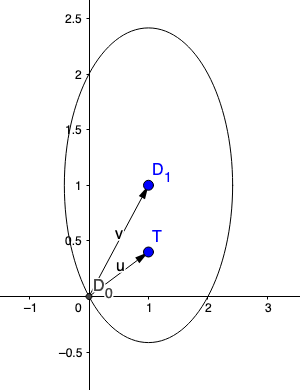
\includegraphics[width=0.4\textwidth]{vectorexample2.png}
    \caption{example in 2D to visualise $\dcs$ in the diagonal basis, the axis
    is in units of $\sigma_{i}$. $\dcs$ can be understood as the pull of
    $\thc$ squared minus two times the dot product of pull of $\thc$ and pull of
    level 1 data. $\dcs = 0$ for the given level 1 shift (in this case
    $\epsilon_1, \epsilon_2 = 1$) is fulfilled at any point on the ellipsoid and
    $\dcs<0$ and $\dcs>0$ refer to the regions inside and outside the ellipsoid
    respectively.}
    \label{fig:vectorexample}
\end{figure}
%
It is clear that the full story of whether a fit is better or not is given not
by a single estimator, but rather on the 3 estimators combined. We now turn to
some example results from level 2 closure tests with the \nfit code to see if we
can say something about the different architectures used in each one.

